\chapter{Resultados}

Os resultados desse trabalho são animadores, pois o resultados obtidos em simulação,
indicam que o sistema tem potencial para ser utilizado em cubesats reais como foi proposto inicialmente,
pois o algoritmo se mostra rápido e robusto, conseguindo indentificar as estrelas presentes no FOV na maioria dos testes,
na tabela ~\ref{tab:tempo_de_execucao_img} é possível observar o tempo em que o algoritmo leva para executar,
a analise da imagem em si o que envolve a aplicação do filtro do borda de Canny, a utilização da transformada de Hough e a detecção de círculos,
e o calculo das relações angulares e geométricas entre as estrelas.

Assim como o tempo de execução, a tabela ~\ref{tab:tempo_de_execucao_db} mostra o tempo de execução da busca no banco de dados,
resultando que esta aplicação realiza a busca para o caso em que o cubesat não possui nenhuma informação anterior sobre a sua posição.

Cabe ressaltar que a terminação final da atitude do cubesat ainda exige a implementação de um algoritmo que relacione a estrela visualizada com a sua posição no espaço.

\begin{table}[ht]
    \centering

    \begin{tabular}{|c|c|c|c|c|}
        \hline
        \textbf{Roll (dec º)} & \textbf{Acensão (dec º)} & \textbf{declinação (dec º)} & \textbf{Tempo analise de imagem (s)} \\ \hline
        0                     & 0                        & 0                           & 1.760                                \\ \hline
        191                   & 170                      & 79                          & 0.770                                \\ \hline
        11                    & 31                       & 44                          & 0.903                                \\ \hline
        92                    & 105                      & 50                          & --                                   \\ \hline
        264                   & 159                      & -63                         & 6.393                                \\ \hline
    \end{tabular}
    \caption{Tempo de execução do algoritmo de analise de imagem, Fonte: Autoria própria}
    \label{tab:tempo_de_execucao_img}
\end{table}

\begin{table}[ht]
    \centering

    \begin{tabular}{|c|c|c|c|c|}
        \hline
        \textbf{Roll (dec º)} & \textbf{Acensão (dec º)} & \textbf{declinação (dec º)} & \textbf{Tempo de busca (s)} \\ \hline
        0                     & 0                        & 0                           & 0.362                       \\ \hline
        191                   & 170                      & 79                          & 3.457                       \\ \hline
        11                    & 31                       & 44                          & 1.132                       \\ \hline
        92                    & 105                      & 50                          & --                          \\ \hline
        264                   & 159                      & -63                         & 2.116                       \\ \hline
    \end{tabular}
    \caption{Tempo de execução da pesquisa no banco de dados, Fonte: Autoria própria}
    \label{tab:tempo_de_execucao_db}
\end{table}

A linha em que o tempo de analise de imagem é -- indica que o sistema não consegui determinar quais estrelas estava sendo analisada no FOV.
Junto a analise de tempo de execução, é realizada a analise de acurácia do sistema,
verificando se o sistema detectou corretamente as estrelas presentes no FOV.

Tal analise é realizada da seguinte forma, primeiramente gera-se um frame aleatório, através do \textit{software} de simulação,
Apos isto o frame é analisado pelo \textit{software} do cubesat que gera uma lista de id sobre as possíveis estrelas, encontradas no FOV.
Com está informação é então criado um novo set de estrelas contendo apenas as estrelas localizadas pelo \textit{software} do cubesat.

Este novo set refinado de estrelas é carregado no \textit{software} de simulação e é então gerado um novo frame, quando então é comparado se o novo frame é compatível com o frame gerado anteriormente,
a Tabela ~\ref{tab:acuracia} mostra os resultados obtidos, pode-se ter 3 resultados distintos:

\begin{itemize}
    \item \textbf{Correto}: o sistema detectou corretamente as estrelas presentes no FOV;
    \item \textbf{Incorreto}: o sistema detectou incorretamente as estrelas presentes no FOV;
    \item \textbf{Inconclusivo}: o sistema não detectou todas as estrelas presentes no FOV.
\end{itemize}

\begin{table}[ht]
    \centering

    \begin{tabular}{|c|c|c|c|c|}
        \hline
        \textbf{Roll (dec º)} & \textbf{Acensão (dec º)} & \textbf{declinação (dec º)} & \textbf{Resultado} \\ \hline
        0                     & 0                        & 0                           & Correto            \\ \hline
        191                   & 170                      & 79                          & Correto            \\ \hline
        11                    & 31                       & 44                          & Incorreto          \\ \hline
        92                    & 105                      & 50                          & Inconclusivo       \\ \hline
        264                   & 159                      & -63                         & Correto            \\ \hline
    \end{tabular}
    \caption{Acurácia do sistema, Fonte: Autoria própria}
    \label{tab:acuracia}
\end{table}

Para reforçar os resultados obtidos as figuras ~\ref{fig:errou}, ~\ref{fig:errou_2D}, ~\ref{fig:errou_3D}, ~\ref{fig:acertou},~\ref{fig:acertou_2D} e ~\ref{fig:acertou_3D} mostram os resultados obtidos para os casos em que o sistema detectou incorretamente e corretamente as estrelas presentes no FOV.

\begin{figure}[H]
    \centering
    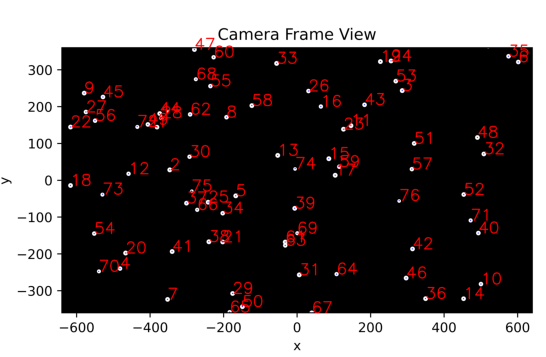
\includegraphics[width=1\textwidth]{images/errou.png}
    \caption{Resultado obtido para o caso em que o sistema detectou incorretamente as estrelas presentes no FOV, Fonte: Autoria própria}
    \label{fig:errou}
\end{figure}

\begin{figure}[H]
    \centering
    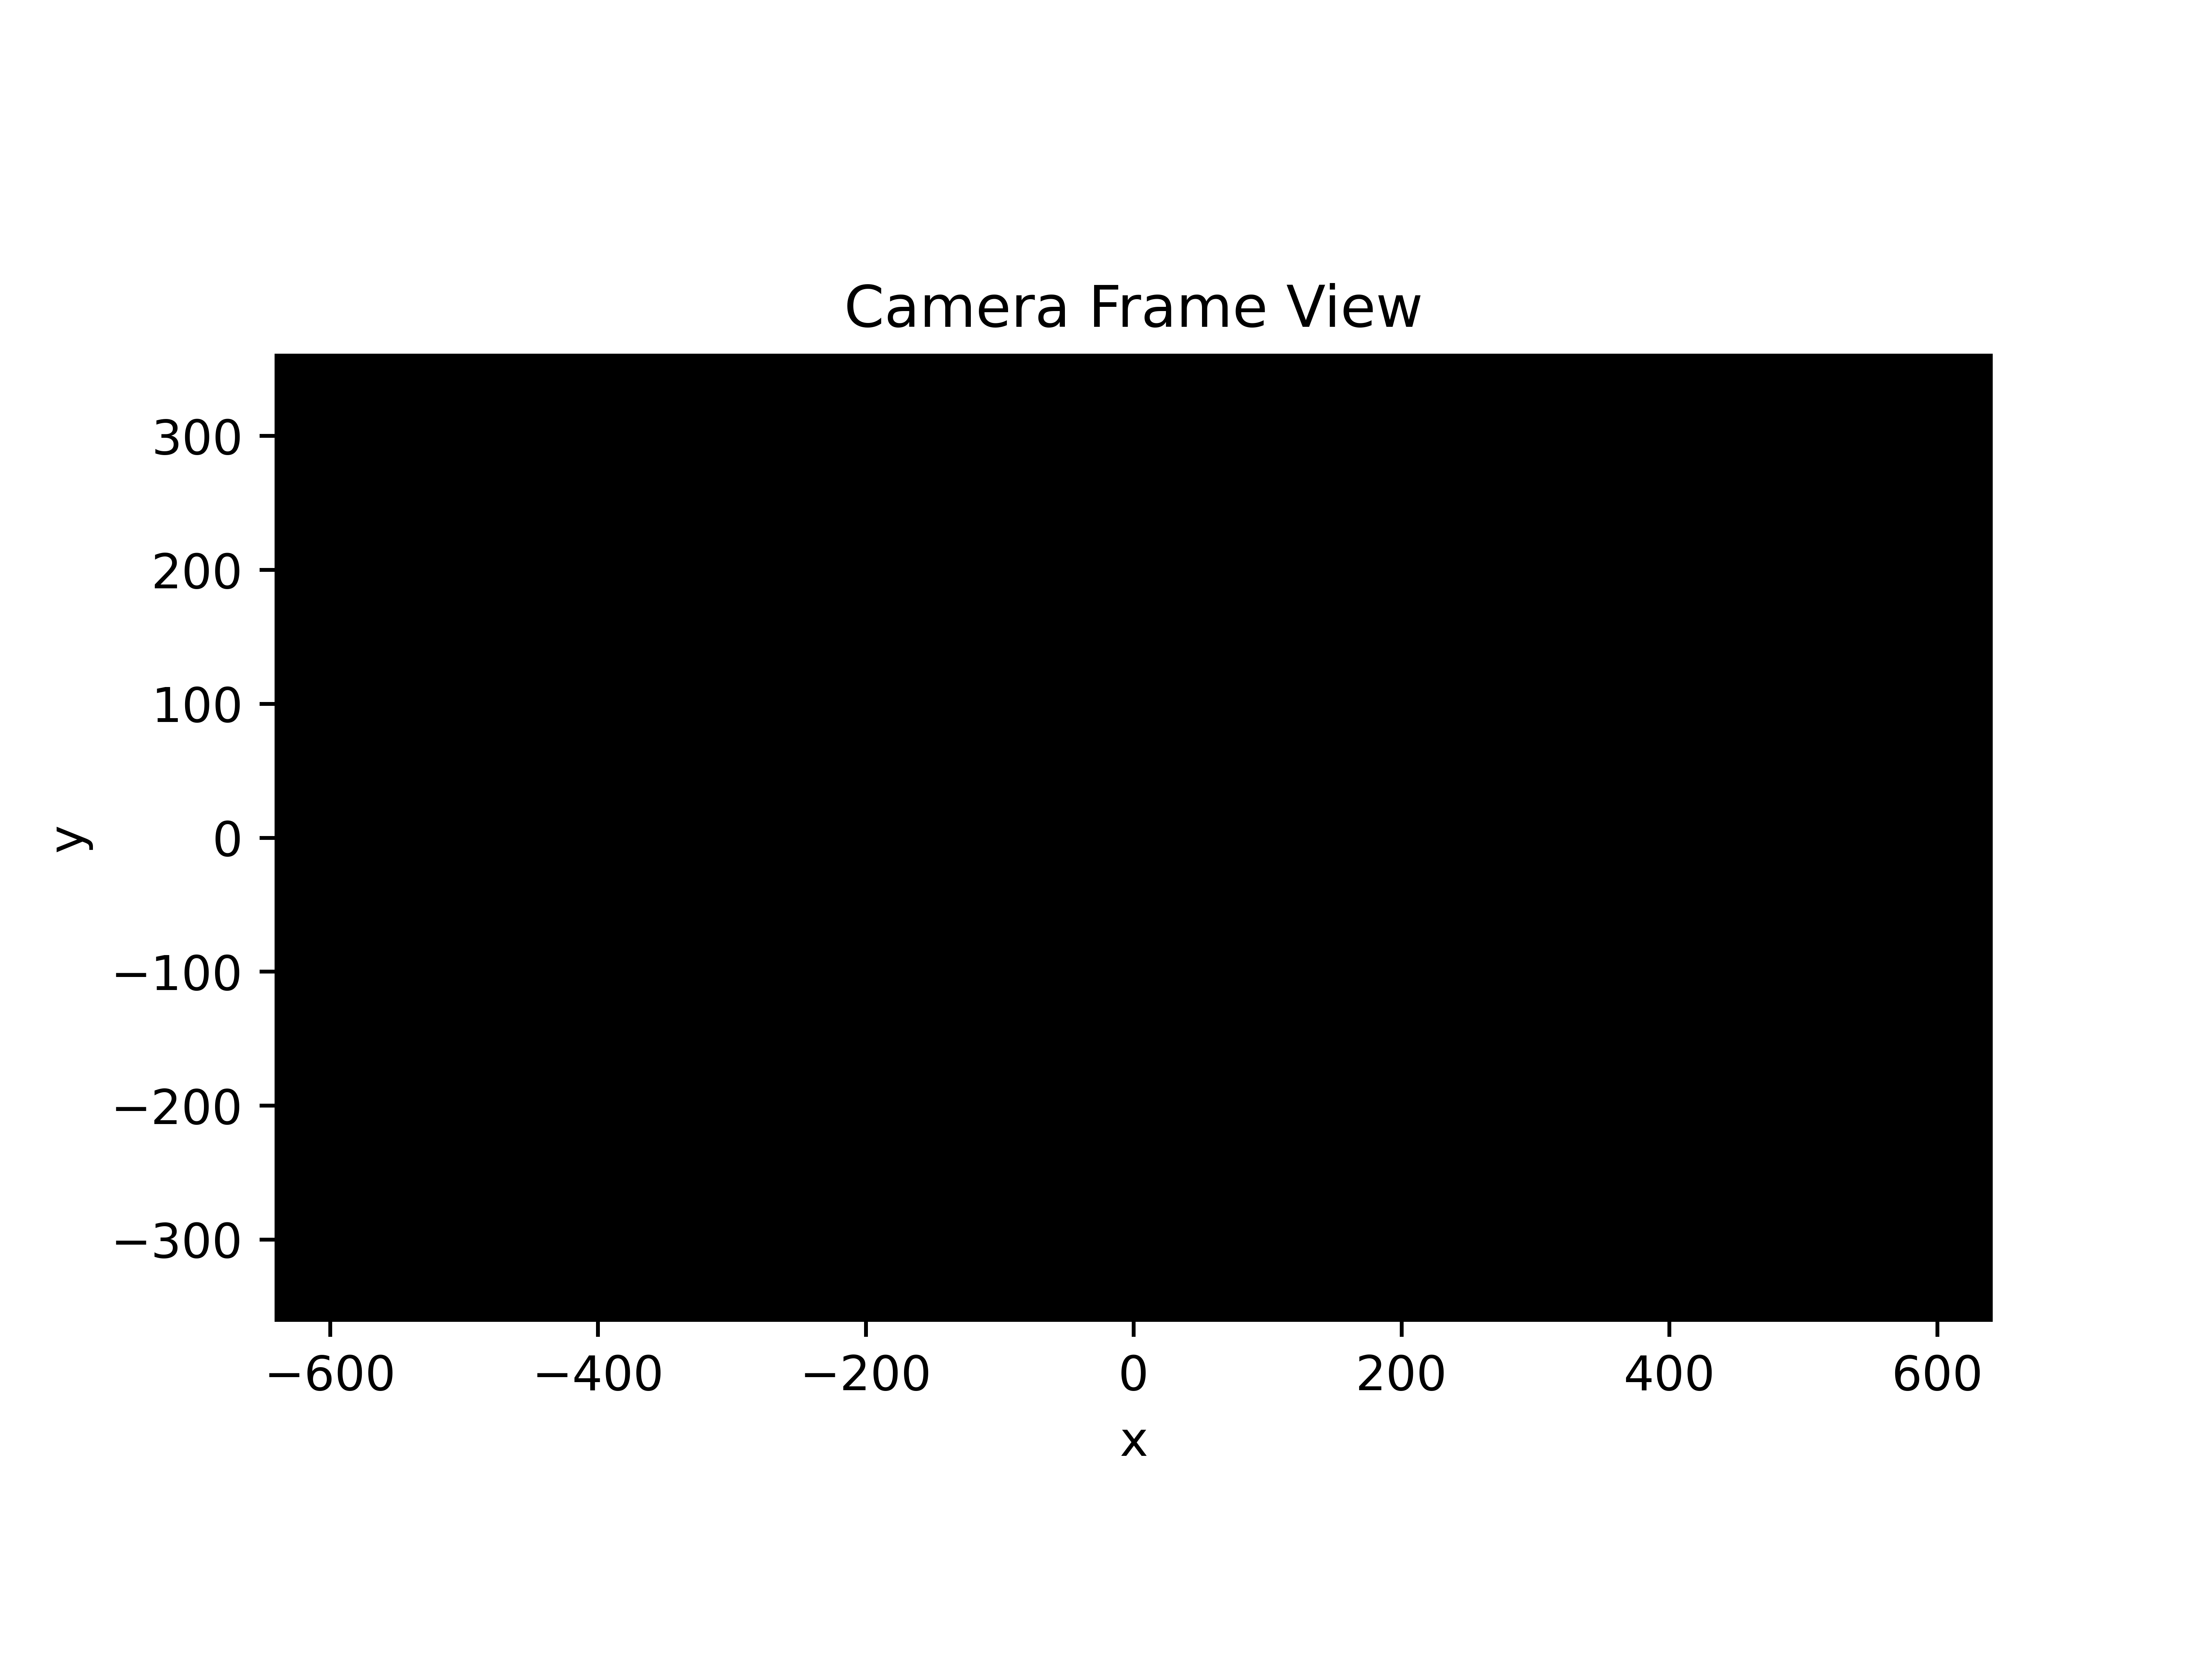
\includegraphics[width=1\textwidth]{images/errou_2D.png}
    \caption{Resultado obtido para o caso em que o sistema detectou incorretamente as estrelas presentes no FOV, Fonte: Autoria própria}
    \label{fig:errou_2D}
\end{figure}

\begin{figure}[H]
    \centering
    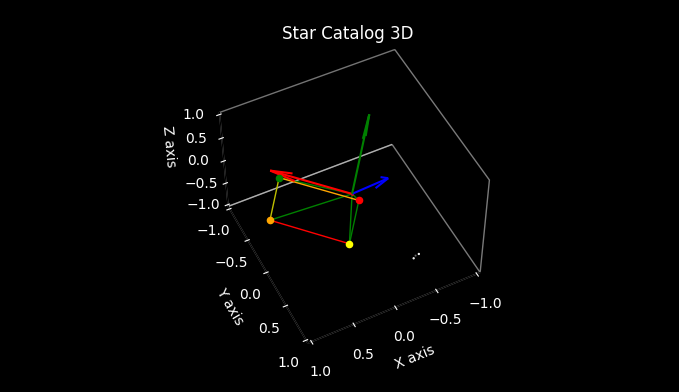
\includegraphics[width=1\textwidth]{images/errou_3D.png}
    \caption{Resultado obtido para o caso em que o sistema detectou incorretamente as estrelas presentes no FOV, Fonte: Autoria própria}
    \label{fig:errou_3D}
\end{figure}

\begin{figure}[H]
    \centering
    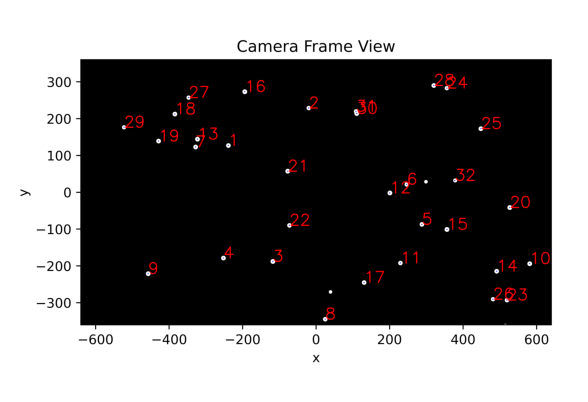
\includegraphics[width=1\textwidth]{images/acertou.png}
    \caption{Resultado obtido para o caso em que o sistema detectou corretamente as estrelas presentes no FOV, Fonte: Autoria própria}
    \label{fig:acertou}
\end{figure}

\begin{figure}[H]
    \centering
    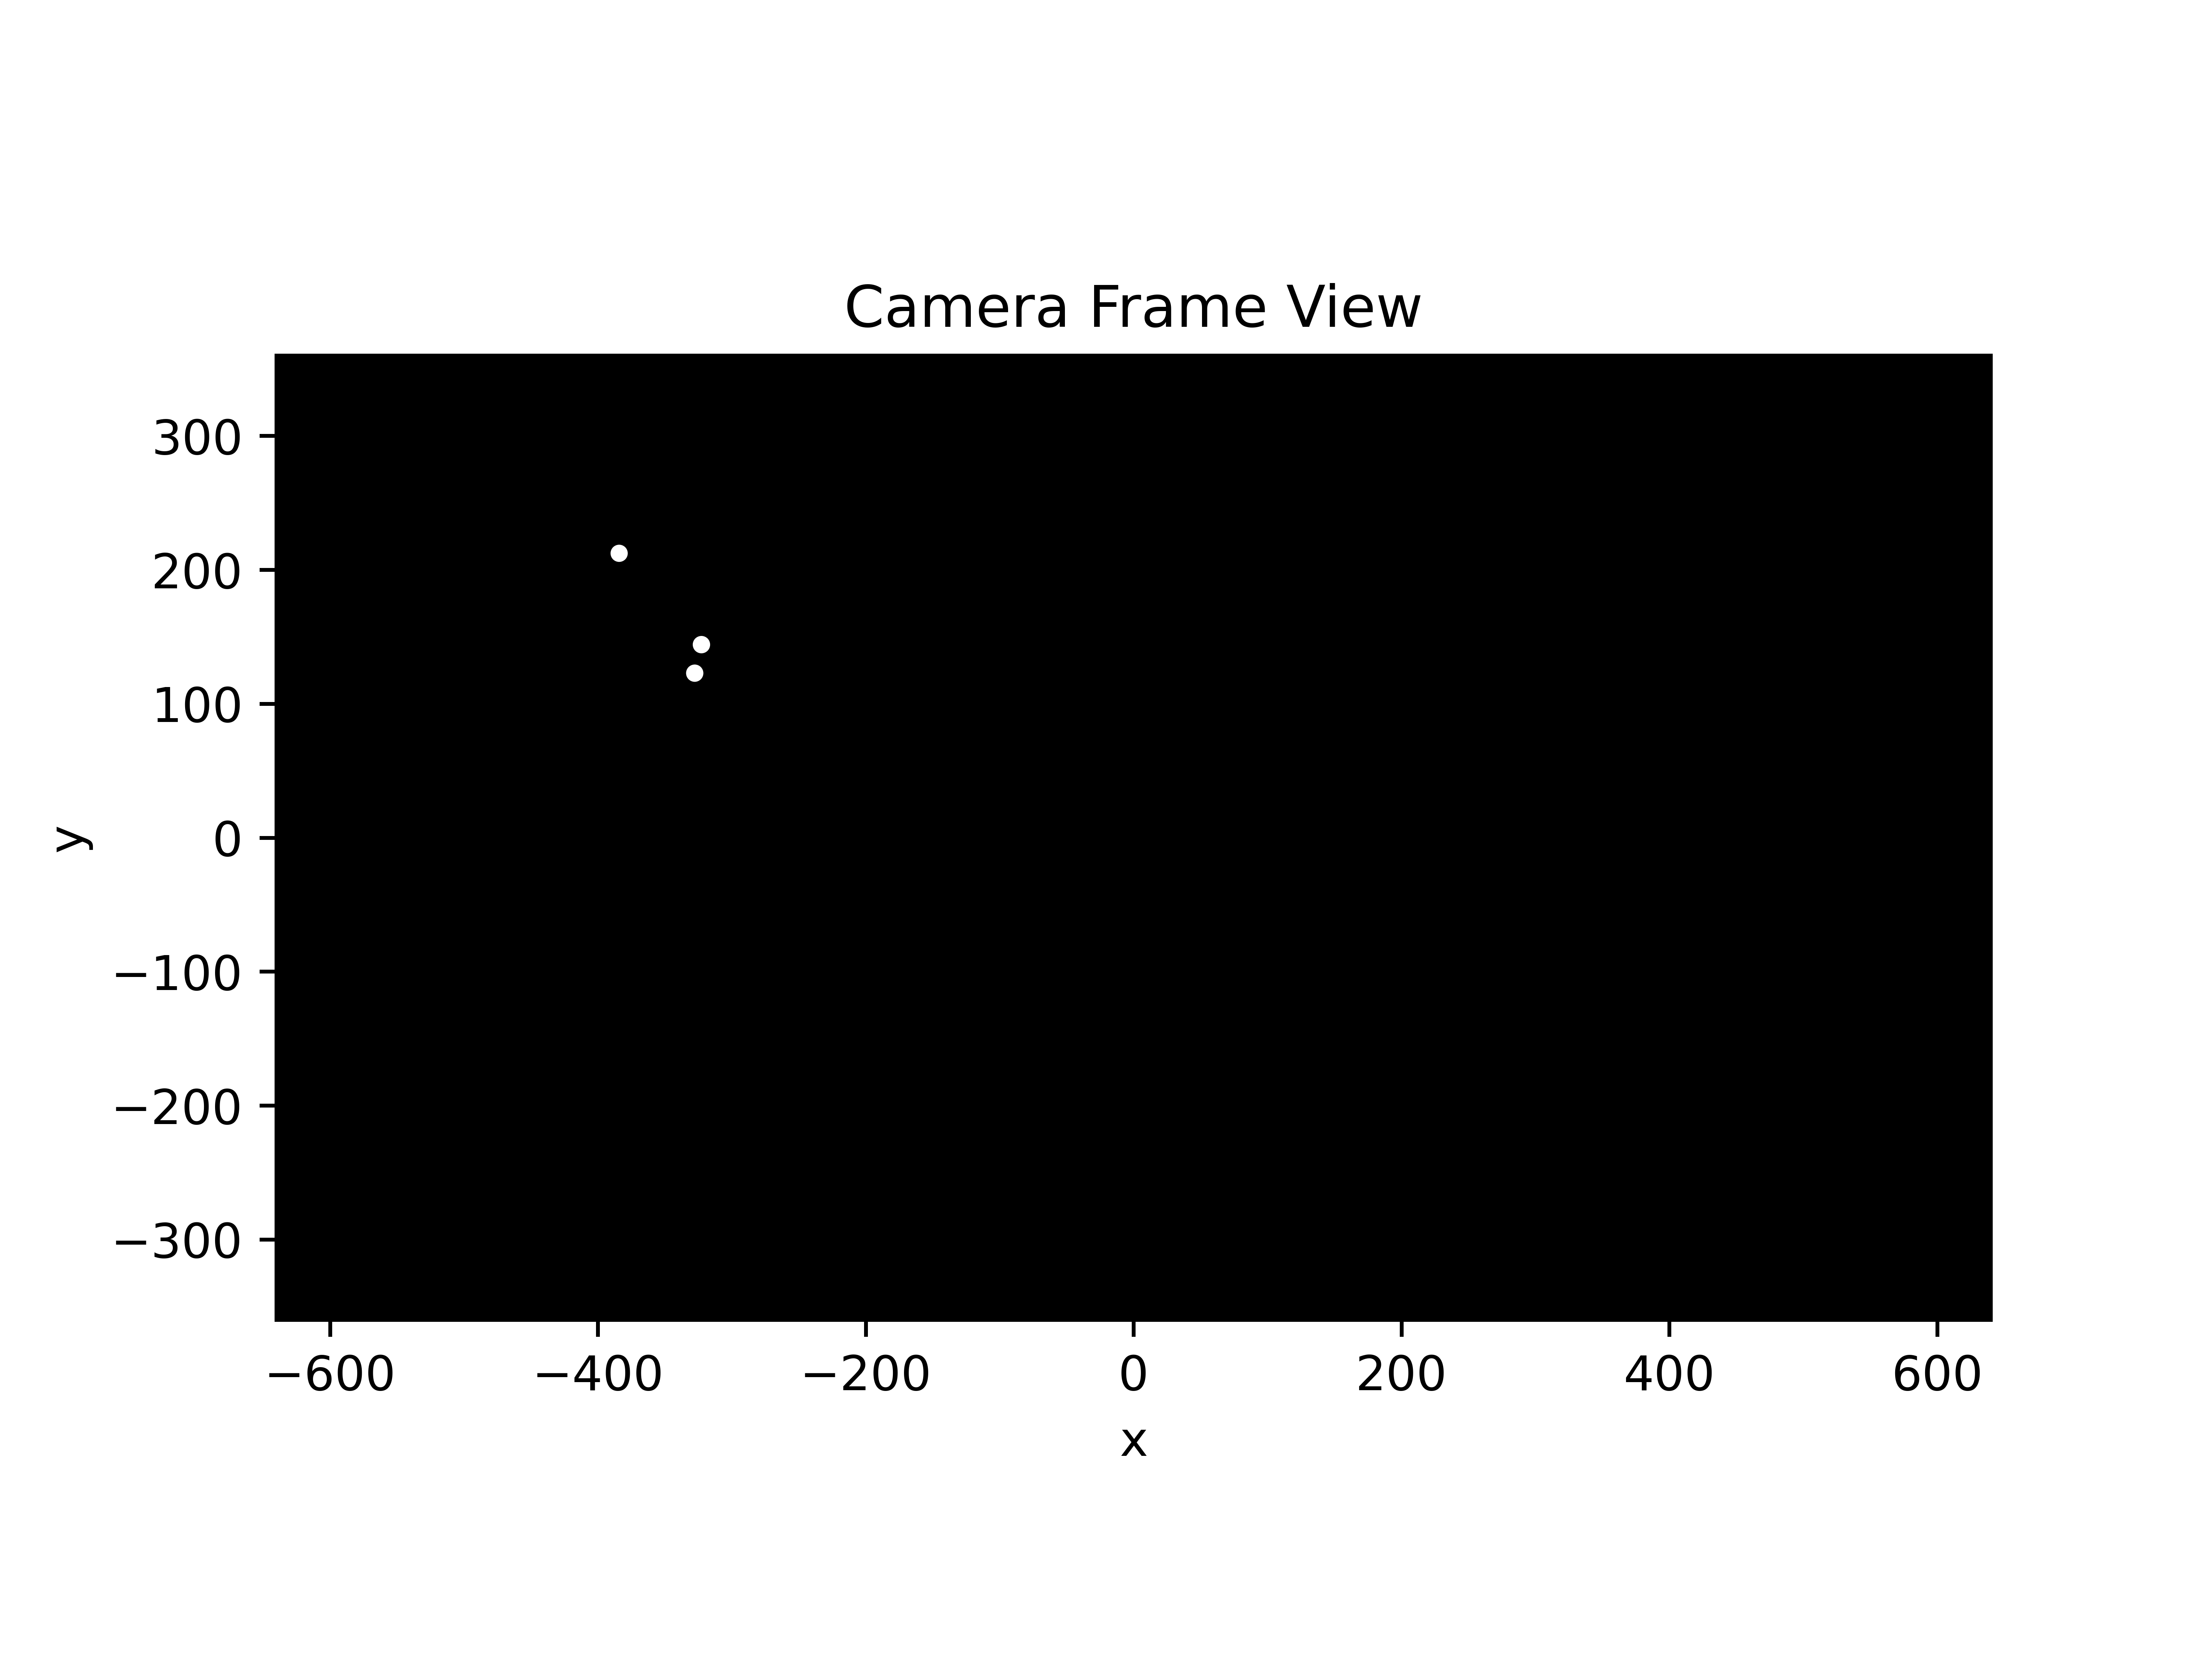
\includegraphics[width=1\textwidth]{images/acertou_2D.png}
    \caption{Resultado obtido para o caso em que o sistema detectou corretamente as estrelas presentes no FOV, Fonte: Autoria própria}
    \label{fig:acertou_2D}
\end{figure}

\begin{figure}[H]
    \centering
    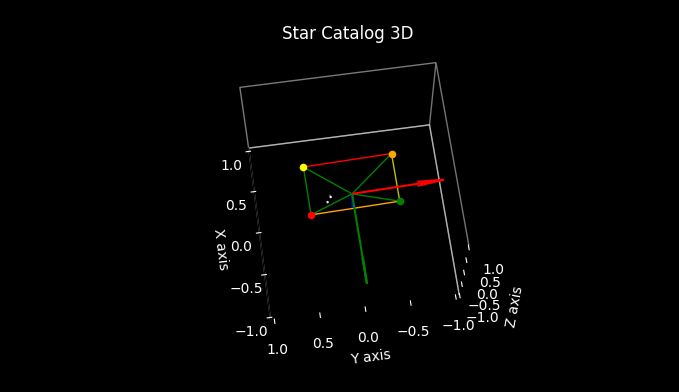
\includegraphics[width=1\textwidth]{images/acertou_3D.png}
    \caption{Resultado obtido para o caso em que o sistema detectou corretamente as estrelas presentes no FOV, Fonte: Autoria própria}
    \label{fig:acertou_3D}
\end{figure}
